\documentclass[11pt,a4paper]{article}

\usepackage[utf8]{inputenc}
\usepackage[T1]{fontenc}
\usepackage{lmodern}
\usepackage{microtype}
\usepackage{geometry}
\usepackage{setspace}
\usepackage{parskip}

\geometry{
    left=2.5cm,
    right=2.5cm,
    top=2.5cm,
    bottom=2.5cm
}
\onehalfspacing
\raggedbottom

\usepackage{graphicx}
\usepackage{float}
\usepackage{subcaption}
\graphicspath{{./}{./assets/}{./images/}}

% Placeholder bila Figure belum tersedia
\newcommand{\testimg}[1]{%
    \IfFileExists{assets/#1}{%
        \includegraphics[width=\textwidth]{assets/#1}%
    }{%
        \fbox{\parbox[c][4cm][c]{0.95\textwidth}{\centering\itshape\small (placeholder: assets/#1)}}%
    }%
}

\usepackage{tikz}
\usetikzlibrary{shapes.geometric, shapes.misc, arrows.meta, positioning, calc, automata, quotes, trees, fit, backgrounds, matrix, chains, decorations.pathreplacing}

\usepackage{listings}
\usepackage{xcolor}

\definecolor{codebg}{HTML}{F7F7F7}
\definecolor{codeframe}{HTML}{DDDDDD}
\definecolor{keyword}{HTML}{005FAF}
\definecolor{comment}{HTML}{6A737D}
\definecolor{string}{HTML}{D73A49}
\definecolor{accent}{HTML}{2E7D32}
\definecolor{warn}{HTML}{C62828}

\lstset{
    basicstyle=\ttfamily\footnotesize,
    keywordstyle=\color{keyword}\bfseries,
    commentstyle=\color{comment}\itshape,
    stringstyle=\color{string},
    numbers=left,
    numberstyle=\tiny\color{gray},
    backgroundcolor=\color{codebg},
    frame=single,
    rulecolor=\color{codeframe},
    breaklines=true,
    tabsize=4,
    showstringspaces=false,
    language=C++,
    aboveskip=1em,
    belowskip=1em,
    extendedchars=true,
    inputencoding=utf8,
    literate=%
        {→}{{$\rightarrow$}}1
        {á}{{\'a}}1 {é}{{\'e}}1 {í}{{\'i}}1 {ó}{{\'o}}1 {ú}{{\'u}}1
}

\usepackage{amsmath}
\usepackage{amssymb}

\usepackage{booktabs}
\usepackage{tabularx}
\usepackage{longtable}
\usepackage{etoolbox}
\usepackage{fancyvrb}

\usepackage{hyperref}
\hypersetup{
    colorlinks=true,
    linkcolor=black,
    urlcolor=keyword,
    citecolor=black,
    pdfauthor={Made Branenda Jordhy, Muhammad Nur Majiid, Jason Edward Salim, Athilla Zaidan Zidna Fann},
    pdftitle={Laporan Milestone 3 - Semantic Analysis - IF2224}
}

% HEADER/FOOTER
\usepackage{fancyhdr}
\pagestyle{fancy}
\fancyhf{}
\setlength{\headheight}{36pt}
\fancyhead[L]{%
    \small\textnormal{School of Electrical Engineering and Informatics}\\[-1pt]
    \small\textnormal{Institut Teknologi Bandung}%
}
\fancyhead[R]{\IfFileExists{assets/LogoITB.png}{
\includegraphics[height=1cm]{assets/LogoITB.png}}{}}
\fancyfoot[L]{\small\textnormal{IF2224 Formal Language and Automata Theory}}
\fancyfoot[R]{\small\thepage}
\renewcommand{\headrulewidth}{0.4pt}
\renewcommand{\footrulewidth}{0.2pt}

% TITLE
\title{
    \vspace{-1.5cm}
    {\Large\textsc{IF2224 Formal Language and Automata Theory}}\\[0.35cm]
    {\LARGE\textbf{Arion Compiler - Milestone 3: Semantic Analysis}}\\[0.3cm]
    \vspace{-0.3cm}
}
\author{}
\date{\today}

\begin{document}

\maketitle
\thispagestyle{empty}

\begin{figure}[H]
    \centering
    \IfFileExists{assets/foto_kelompok.png}{%
        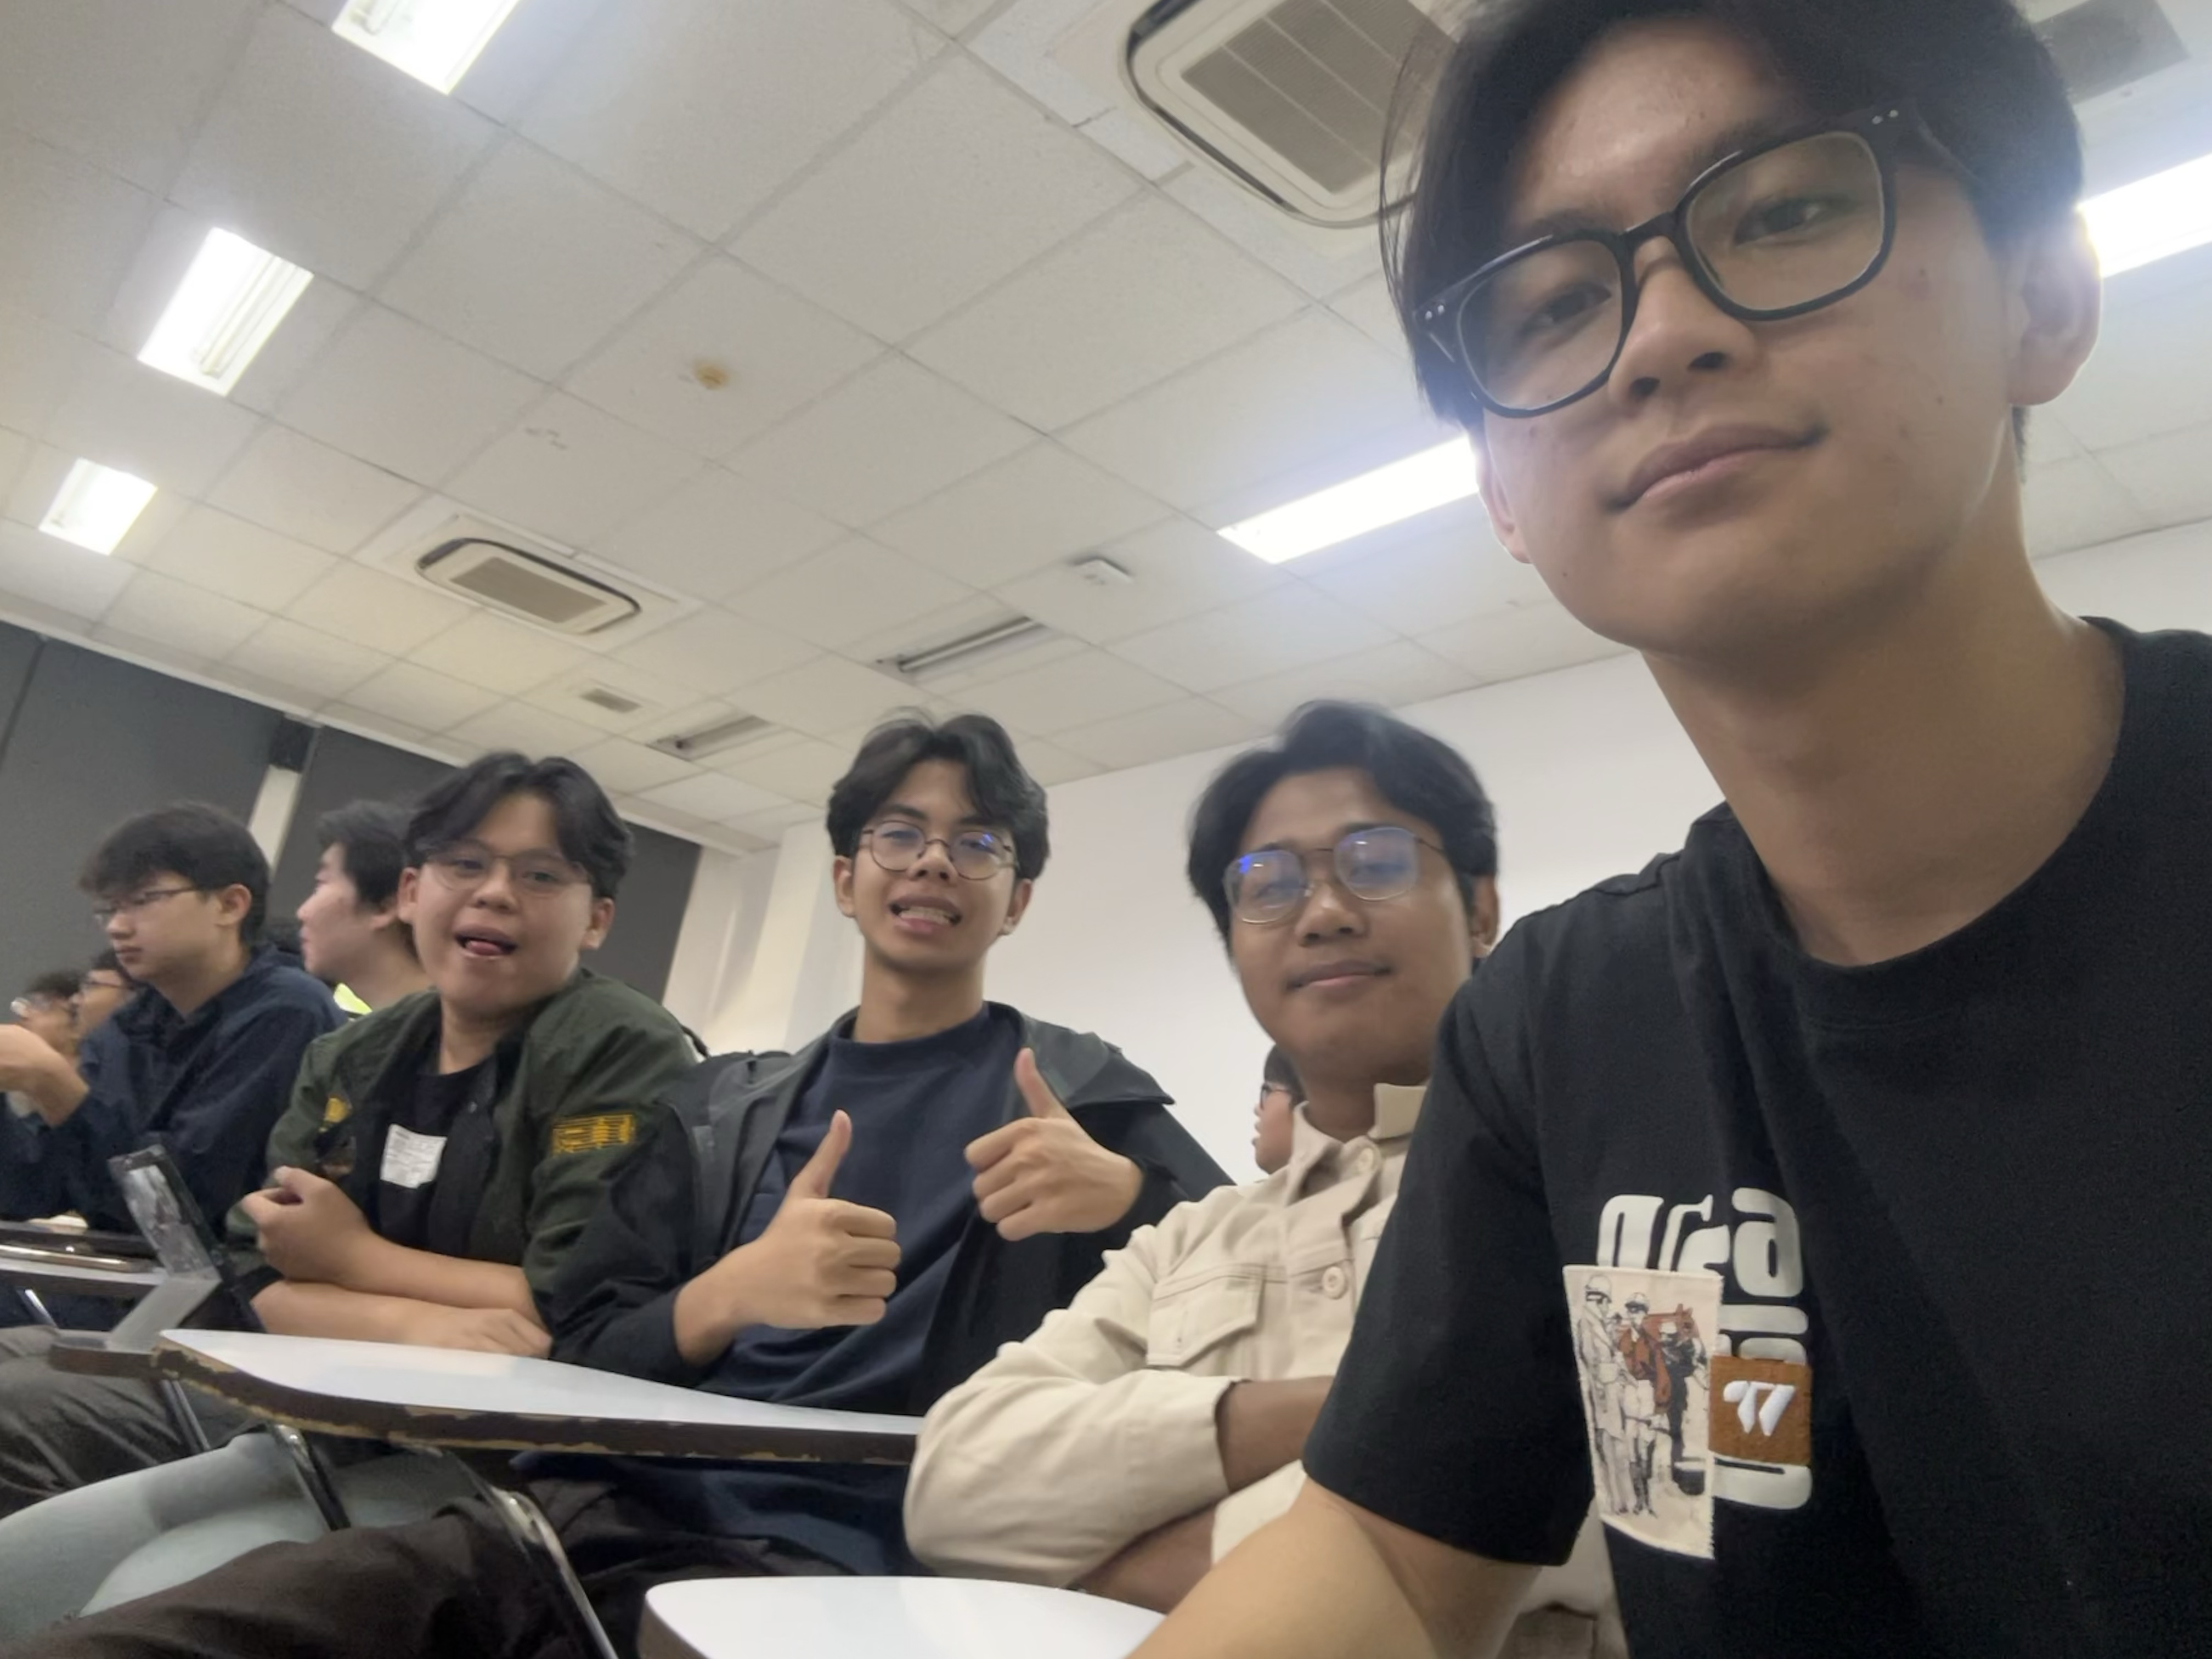
\includegraphics[width=0.6\textwidth]{assets/foto_kelompok.png}%
    }{%
        \vspace{4cm}
    }
\end{figure}

\vspace{1cm}
\begin{center}
    \textbf{Made Branenda Jordhy} - 13524026 \\[0.15cm]
    \textbf{Muhammad Nur Majiid} - 13524028 \\[0.15cm]
    \textbf{Jason Edward Salim} - 13524034 \\[0.15cm]
    \textbf{Athilla Zaidan Zidna Fann} - 13524068
\end{center}

\vspace{3cm}
\begin{center}
    {\large\textbf{School of Electrical Engineering and Informatics}}\\[0.1cm]
    {\large\textbf{Institut Teknologi Bandung}}\\[0.1cm]
    {\large\textbf{Semester II 2025/2026}}\\[0.1cm]
\end{center}

\newpage
\tableofcontents
\newpage

% =======================================================================
\section{Theoretical Background}

\subsection{Semantic Analysis}

\textit{Semantic analysis} adalah fase ketiga dalam pipeline kompilasi, setelah
\textit{lexical analysis} (Milestone~1) dan \textit{syntax analysis}
(Milestone~2). Pada tahap ini, parse tree yang sudah dibangun parser ditelusuri
ulang untuk memverifikasi \textbf{makna} program, bukan lagi sekadar bentuk
sintaktiknya. Pengecekan yang dilakukan meliputi empat aspek besar:

\begin{itemize}
    \item \textbf{Type checking} - memastikan operator dan operand memiliki
          tipe yang kompatibel (mis.\ tidak menjumlahkan \texttt{integer} dengan
          \texttt{string}).
    \item \textbf{Symbol table management} - memastikan setiap identifier
          dideklarasikan sebelum digunakan dan tidak dideklarasikan ulang dalam
          cakupan yang sama.
    \item \textbf{Scope resolution} - menentukan validitas akses variabel
          berdasarkan hierarki blok kode (global vs lokal vs nested).
    \item \textbf{Control flow validation} - memastikan struktur alur kontrol
          logis (kondisi \texttt{if}/\texttt{while} bertipe \texttt{boolean},
          dsb.).
\end{itemize}

Sebagai keluaran, semantic analyzer menghasilkan \textbf{Decorated Abstract
Syntax Tree (AST)} - yaitu AST yang setiap nodenya dianotasi dengan informasi
tambahan seperti tipe data hasil ekspresi, indeks ke symbol table, dan
\textit{lexical level} tempat node tersebut berada.

\subsection{Abstract Syntax Tree (AST)}

\textit{Abstract Syntax Tree} adalah bentuk ringkas dari parse tree yang hanya
menyimpan informasi struktural yang relevan secara semantis. Parse tree masih
memuat seluruh non-terminal antara (\texttt{<simple-expression>},
\texttt{<term>}, dst.) serta token sintaktis (\texttt{begin}, \texttt{end},
\texttt{;}, \texttt{(}, \texttt{)}) yang berguna untuk pengecekan grammar tetapi
tidak diperlukan untuk analisis makna. AST membuang informasi tersebut dan
mempertahankan hanya hubungan antar operator-operand.

Figure~\ref{fig:ast-vs-parse} memperlihatkan perbedaan tersebut untuk ekspresi
sederhana \texttt{7 + (2 + 3)}: parse tree memuat tujuh tingkat non-terminal
sebelum mencapai daun, sedangkan AST cukup direpresentasikan oleh tiga node.

\begin{figure}[H]
\centering
\begin{tikzpicture}[
    every node/.style={font=\footnotesize},
    n/.style={draw, rounded corners=2pt, fill=codebg, inner sep=3pt},
    arr/.style={-{Stealth[length=2mm]}, thick}
]
    % ===== AST (kiri) =====
    \node[n] (ap)  at (0, 0)   {\texttt{+}};
    \node[n] (a7)  at (-1.2, -1.2) {\texttt{7}};
    \node[n] (ap2) at ( 1.2, -1.2) {\texttt{+}};
    \node[n] (a2)  at ( 0.3, -2.4) {\texttt{2}};
    \node[n] (a3)  at ( 2.1, -2.4) {\texttt{3}};
    \draw[arr] (ap) -- (a7);
    \draw[arr] (ap) -- (ap2);
    \draw[arr] (ap2) -- (a2);
    \draw[arr] (ap2) -- (a3);
    \node[font=\small\bfseries] at (0.45, 0.9) {AST};

    % ===== Parse tree (kanan) =====
    \begin{scope}[xshift=8cm, yshift=0.5cm]
        \node[n] (e)  at (0, 0)     {\texttt{<expr>}};
        \node[n] (t1) at (-2.4, -1) {\texttt{<term>}};
        \node[n] (op) at ( 0,    -1) {\texttt{+}};
        \node[n] (t2) at ( 2.4, -1) {\texttt{<term>}};
        \node[n] (f1) at (-2.4, -2) {\texttt{<factor>}};
        \node[n] (n7) at (-2.4, -3) {\texttt{7}};
        \node[n] (f2) at ( 2.4, -2) {\texttt{<factor>}};
        \node[n] (lp) at ( 1.4, -3) {\texttt{(}};
        \node[n] (e2) at ( 2.4, -3) {\texttt{<expr>}};
        \node[n] (rp) at ( 3.4, -3) {\texttt{)}};
        \node[n] (s2) at ( 2.4, -4) {\texttt{2+3}};
        \draw[arr] (e) -- (t1);
        \draw[arr] (e) -- (op);
        \draw[arr] (e) -- (t2);
        \draw[arr] (t1) -- (f1);
        \draw[arr] (f1) -- (n7);
        \draw[arr] (t2) -- (f2);
        \draw[arr] (f2) -- (lp);
        \draw[arr] (f2) -- (e2);
        \draw[arr] (f2) -- (rp);
        \draw[arr] (e2) -- (s2);
        \node[font=\small\bfseries] at (0.5, 0.9) {Parse Tree};
    \end{scope}
\end{tikzpicture}
\caption{Perbandingan AST dan parse tree untuk ekspresi \texttt{7 + (2 + 3)}.
AST membuang non-terminal antara dan token sintaktis, menyisakan hanya
operator-operand yang relevan secara semantis.}
\label{fig:ast-vs-parse}
\end{figure}

\subsection{Decorated AST}

Decorated AST adalah AST hasil tahap semantik di mana setiap node telah
dilengkapi dengan \textit{atribut} hasil evaluasi. Atribut minimal yang
ditanamkan pada implementasi Arion adalah:

\begin{itemize}
    \item \texttt{dataType} - tipe data akhir dari ekspresi node tersebut
          (mis.\ \texttt{integer}, \texttt{real}, \texttt{boolean}).
    \item \texttt{tabIndex} - indeks ke entri \texttt{tab} pada symbol table
          (untuk identifier, ini adalah deklarasi yang di-\textit{resolve}).
    \item \texttt{lexLevel} - tingkat \textit{lexical scope} tempat node berada
          (0 = global, 1 = dalam prosedur/fungsi tingkat-1, dst.).
\end{itemize}

Anotasi inilah yang akan menjadi masukan utama untuk tahap berikutnya
(\textit{intermediate representation generation} dan \textit{code generation}).

\subsection{Attributed Grammar dan Syntax-Directed Translation}

\textit{Attributed grammar} adalah CFG yang dilengkapi dengan \textit{atribut}
pada setiap simbol dan \textit{semantic rule} yang menentukan bagaimana atribut
tersebut dihitung. Untuk pengerjaan Milestone~3 ini, atribut yang digunakan
bersifat \textbf{synthesized} (dihitung dari atribut child ke parent) dengan
beberapa atribut \textbf{inherited} (mis.\ \texttt{lexLevel}) yang diturunkan
dari parent ke child. Karakteristik ini menjadikannya \textit{L-Attributed
Grammar}, yang cocok dievaluasi dengan satu kali penelusuran DFS dari kiri ke
kanan.

Tabel~\ref{tab:semrules} memperlihatkan contoh aturan semantik yang digunakan
pada beberapa produksi penting.

\renewcommand{\arraystretch}{1.15}
\begin{table}[H]
\centering
\footnotesize
\begin{tabularx}{\textwidth}{l X}
\toprule
\textbf{Production Rule} & \textbf{Semantic Rule} \\
\midrule
\texttt{<assignment-statement>} $\to$ \texttt{ID := <expr>} &
    \texttt{node = new AssignNode(new VarNode(ID.lexeme), expr.node)} \\
\texttt{<expression>} $\to$ \texttt{<simple-expr>} \texttt{+} \texttt{<term>} &
    \texttt{node = new BinOpNode('+', simple\_expr.node, term.node)} \\
\texttt{<expression>} $\to$ \texttt{<simple-expr>} &
    \texttt{node = simple\_expr.node} \\
\texttt{<factor>} $\to$ \texttt{INTCON} &
    \texttt{node = new NumberNode(INTCON.value, isReal=false)} \\
\texttt{<factor>} $\to$ \texttt{ID} &
    \texttt{node = new VarNode(ID.lexeme)} \\
\texttt{<term>} $\to$ \texttt{<factor>} &
    \texttt{node = factor.node} \\
\texttt{<factor>} $\to$ \texttt{STRING\_LITERAL} &
    \texttt{node = new StringNode(STRING\_LITERAL.value)} \\
\texttt{<procedure-call>} $\to$ \texttt{ID ( <params> )} &
    \texttt{node = new CallNode(ID.lexeme, params.nodes)} \\
\bottomrule
\end{tabularx}
\caption{Contoh \textit{semantic rule} yang digunakan untuk konstruksi AST.}
\label{tab:semrules}
\end{table}
\renewcommand{\arraystretch}{1.05}

\subsection{Symbol Table: \texttt{tab}, \texttt{btab}, dan \texttt{atab}}

Sesuai spesifikasi, symbol table pada Arion dipecah menjadi tiga tabel terpisah
yang saling merujuk:

\begin{itemize}
    \item \textbf{\texttt{tab}} - tabel identifier utama. Menyimpan
          konstanta, variabel, tipe, prosedur, fungsi, dan field record dengan
          atribut \texttt{id, link, obj, type, ref, nrm, lev, adr}.
    \item \textbf{\texttt{btab}} - \textit{block table}. Setiap entri
          merepresentasikan satu blok (program global, prosedur, fungsi, atau
          definisi record). Atribut: \texttt{last, lpar, psze, vsze}.
    \item \textbf{\texttt{atab}} - \textit{array table}. Setiap entri
          merepresentasikan tipe komposit array atau subrange. Atribut:
          \texttt{xtyp, etyp, eref, low, high, elsz, size}.
\end{itemize}

Figure~\ref{fig:symtab-arch} memperlihatkan hubungan antar ketiga tabel.

\begin{figure}[H]
\centering
\resizebox{0.95\textwidth}{!}{%
\begin{tikzpicture}[
    every node/.style={font=\footnotesize},
    tbl/.style={draw, fill=codebg, rounded corners=3pt, minimum width=4cm,
                minimum height=2.2cm, align=center},
    arr/.style={-{Stealth[length=2.5mm]}, thick, color=keyword},
    lbl/.style={font=\scriptsize\itshape, fill=white, inner sep=1pt}
]
    \node[tbl] (tab)  at (0, 0)
        {\textbf{tab}\\[2pt]\scriptsize identifier table\\[4pt]
         \scriptsize\texttt{id, link, obj, type,}\\
         \scriptsize\texttt{ref, nrm, lev, adr}};
    \node[tbl] (btab) at (6, 1.2)
        {\textbf{btab}\\[2pt]\scriptsize block table\\[4pt]
         \scriptsize\texttt{last, lpar,}\\
         \scriptsize\texttt{psze, vsze}};
    \node[tbl] (atab) at (6, -1.8)
        {\textbf{atab}\\[2pt]\scriptsize array/range table\\[4pt]
         \scriptsize\texttt{xtyp, etyp, eref,}\\
         \scriptsize\texttt{low, high, elsz, size}};

    \draw[arr] (tab.north east) to[bend left=15]
        node[lbl, above] {\texttt{ref} (procedure/record)} (btab.west);
    \draw[arr] (tab.south east) to[bend right=15]
        node[lbl, below] {\texttt{ref} (array/subrange)} (atab.west);
    \draw[arr] (btab.south west) to[bend left=18]
        node[lbl, sloped, above] {\texttt{last/lpar} $\to$ \texttt{tab}}
        (tab.east);
\end{tikzpicture}}
\caption{Hubungan antara \texttt{tab}, \texttt{btab}, dan \texttt{atab}. Field
\texttt{ref} pada \texttt{tab} mengarah ke entri \texttt{btab} (untuk
prosedur/fungsi/record) atau \texttt{atab} (untuk array/subrange).}
\label{fig:symtab-arch}
\end{figure}

Setiap blok membentuk \textbf{linked list} dari deklarasi yang dimilikinya:
\texttt{btab[i].last} menunjuk ke entri terakhir di \texttt{tab} yang termasuk
blok ke-\texttt{i}, dan masing-masing entri pada \texttt{tab} memiliki kolom
\texttt{link} yang menunjuk ke deklarasi sebelumnya dalam blok yang sama.
Penambahan deklarasi bersifat \textit{push} ke kepala list - lihat
Figure~\ref{fig:linked-list}.

\begin{figure}[H]
\centering
\begin{tikzpicture}[
    every node/.style={font=\scriptsize},
    box/.style={draw, fill=codebg, rounded corners=2pt, minimum width=1.6cm,
                minimum height=0.7cm},
    head/.style={draw, fill=accent!12, rounded corners=2pt, minimum width=2.1cm,
                minimum height=0.8cm},
    arr/.style={-{Stealth[length=2.2mm]}, thick}
]
    \node[head] (h)   at (0,    0) {\texttt{btab[i].last}};
    \node[box]  (e3)  at (3,    0) {\texttt{tab[36] c}};
    \node[box]  (e2)  at (5.5,  0) {\texttt{tab[35] b}};
    \node[box]  (e1)  at (8,    0) {\texttt{tab[34] a}};
    \node[box]  (nil) at (10.5, 0) {\texttt{0 (nil)}};

    \draw[arr] (h)   -- (e3);
    \draw[arr] (e3)  -- node[above]{\texttt{link}} (e2);
    \draw[arr] (e2)  -- node[above]{\texttt{link}} (e1);
    \draw[arr] (e1)  -- node[above]{\texttt{link}} (nil);
\end{tikzpicture}
\caption{Tiap blok memuat \textit{linked list} deklarasinya. Field \texttt{link}
pada setiap entri \texttt{tab} menunjuk ke deklarasi sebelumnya dalam blok
yang sama; entri terbaru selalu ditambahkan di kepala list lewat
\texttt{btab[i].last}.}
\label{fig:linked-list}
\end{figure}

\subsection{Scope Resolution dan Display}

Scope dikelola dengan \textbf{stack \texttt{display}} yang menyimpan indeks
\texttt{btab} dari setiap level cakupan yang sedang aktif. Pencarian
identifier (\textit{lookup}) dimulai dari level terdalam dan menelusuri ke
level paling luar (level 0 = global, termasuk \textit{reserved words} dan
\textit{predefined identifier}).

Figure~\ref{fig:scope-stack} memperlihatkan keadaan stack \texttt{display}
ketika analyzer berada di dalam prosedur \texttt{Inner} yang bersarang di
dalam prosedur \texttt{Outer}.

\begin{figure}[H]
\centering
\begin{tikzpicture}[
    every node/.style={font=\footnotesize},
    block/.style={draw, fill=codebg, minimum width=4cm, minimum height=0.8cm,
                  rounded corners=2pt},
    activeblock/.style={draw, fill=accent!12, minimum width=4cm, minimum height=0.8cm,
                       rounded corners=2pt, very thick},
    lbl/.style={font=\scriptsize\itshape, text=comment}
]
    % Display stack
    \node[activeblock] (l2) at (0, 0)    {level 2: \texttt{Inner} (\texttt{btab[2]})};
    \node[block]       (l1) at (0, -1)   {level 1: \texttt{Outer} (\texttt{btab[1]})};
    \node[block]       (l0) at (0, -2)   {level 0: global (\texttt{btab[0]})};

    \node[lbl] at (4.0, 0)    {\textbf{top} -- pencarian mulai di sini};
    \node[lbl] at (4.0, -1)   {parent procedure};
    \node[lbl] at (4.0, -2)   {global + predefined};

    % Brace + arrow showing search direction
    \draw[->, very thick, color=keyword]
        ($(l2.west)+(-0.6, 0)$) -- ($(l0.west)+(-0.6, 0)$)
        node[midway, left, font=\scriptsize\itshape, text=keyword, align=center]
        {arah\\lookup};
\end{tikzpicture}
\caption{Stack \texttt{display} ketika analyzer berada dalam \texttt{Inner}.
Lookup identifier menelusuri stack dari level tertinggi (terdalam) ke level
0 (global).}
\label{fig:scope-stack}
\end{figure}

\subsection{Visitor Pattern dan Traversal DFS}

Setiap jenis node AST memiliki fungsi \texttt{visit\_<node>} yang dipanggil
secara rekursif. Fungsi visit ini bertugas:

\begin{enumerate}
    \item Memanggil visit pada child node-nya (penelusuran DFS).
    \item Mengakses atau memperbarui symbol table (push/pop block, enter
          identifier, lookup).
    \item Menghitung atribut atau tipe semantik node.
    \item Menanamkan anotasi pada node (\texttt{dataType, tabIndex, lexLevel}).
\end{enumerate}

\subsection{Type Compatibility}

\textit{Type compatibility rule} menentukan kapan dua tipe dapat digunakan
bersama dalam ekspresi atau \textit{assignment}. Dua jenis kompatibilitas yang
dibedakan:

\begin{itemize}
    \item \textbf{Compatible} - dua tipe dapat dibandingkan atau dioperasikan
          (mis.\ pada operator relasional).
    \item \textbf{Assignment-compatible} - tipe sumber dapat dikonversi ke
          tipe tujuan pada operasi \texttt{:=}, misalnya \texttt{integer} dapat
          di-assign ke variabel \texttt{real}.
\end{itemize}

Aturan dasar yang digunakan dirangkum pada Tabel~\ref{tab:type-rules} di
Bagian Implementasi.

% =======================================================================
\section{Design and Implementation}

\subsection{Overview Pipeline}

Tahap semantik dijalankan sebagai kelanjutan langsung dari parser
Milestone~2. Pipeline kompilasi sekarang terdiri atas lima komponen yang
dirangkai pada \texttt{src/main.cpp}.

\begin{figure}[H]
\centering
\resizebox{\textwidth}{!}{%
\begin{tikzpicture}[
    every node/.style={font=\small},
    src/.style={rectangle, draw, fill=codebg, rounded corners=2pt,
                minimum width=2.6cm, minimum height=0.9cm, align=center},
    proc/.style={rectangle, draw, fill=yellow!12, rounded corners=2pt,
                 minimum width=2.6cm, minimum height=0.9cm, align=center},
    sem/.style={rectangle, draw, fill=accent!15, rounded corners=2pt,
                 minimum width=2.6cm, minimum height=0.9cm, align=center},
    deco/.style={rectangle, draw, fill=keyword!10, rounded corners=2pt,
                minimum width=2.6cm, minimum height=0.9cm, align=center},
    arr/.style={-{Stealth[length=2.5mm]}, thick}
]
    \node[src]                       (src)  at (0,    0) {\texttt{program.txt}};
    \node[proc, right=0.6cm of src]  (lex)  {Lexer};
    \node[src,  right=0.6cm of lex]  (tok)  {Tokens};
    \node[proc, right=0.6cm of tok]  (par)  {Parser};
    \node[src,  right=0.6cm of par]  (pt)   {Parse Tree};
    \node[proc, below=1cm of pt]     (bld)  {AST Builder};
    \node[src,  left=0.6cm of bld]   (ast)  {AST};
    \node[sem,  left=0.6cm of ast, minimum width=3.0cm]   (sem)  {Semantic Analyzer};
    \node[deco, left=0.6cm of sem, minimum width=3.4cm]   (dec)  {Decorated AST + Symtab};

    \draw[arr] (src) -- (lex);
    \draw[arr] (lex) -- (tok);
    \draw[arr] (tok) -- (par);
    \draw[arr] (par) -- (pt);
    \draw[arr] (pt)  -- (bld);
    \draw[arr] (bld) -- (ast);
    \draw[arr] (ast) -- (sem);
    \draw[arr] (sem) -- (dec);
\end{tikzpicture}}
\caption{Pipeline kompilasi Arion sampai Milestone~3. Komponen baru yang
ditambahkan pada milestone ini adalah \textit{AST Builder} dan \textit{Semantic
Analyzer}, keduanya menghasilkan \textbf{Decorated AST} beserta isi symbol
table sebagai keluaran tahap semantik.}
\label{fig:pipeline}
\end{figure}

Source code milestone ini terbagi menjadi modul berikut:

\begin{itemize}
    \item \texttt{src/header/ast.hpp} \& \texttt{src/lib/ast.cpp} -
          definisi dan implementasi node AST serta \texttt{buildAST()} yang
          mengkonversi parse tree menjadi AST.
    \item \texttt{src/header/symtab.hpp} \& \texttt{src/lib/symtab.cpp} -
          definisi \texttt{SymbolTable} (tab/btab/atab) dan kelas
          \texttt{SemanticAnalyzer} dengan seluruh visit functions.
    \item \texttt{src/main.cpp} - menyambung lexer, parser, AST builder, dan
          semantic analyzer menjadi satu pipeline interaktif.
\end{itemize}

\subsection{AST Node Hierarchy}

AST direpresentasikan oleh basis struct \texttt{ASTNode} yang diperluas oleh
berbagai subtipe. Setiap subtipe menyimpan informasi spesifik untuk konstruksi
bahasa tertentu. Figure~\ref{fig:ast-hier} memperlihatkan kategorisasi node.

\begin{figure}[H]
\centering
\begin{tikzpicture}[
    every node/.style={font=\scriptsize},
    root/.style={draw, rounded corners=2pt, fill=accent!15, inner sep=4pt,
                 minimum width=2cm, minimum height=0.6cm, align=center},
    group/.style={draw, rounded corners=2pt, fill=yellow!15, inner sep=4pt,
                  minimum width=2.4cm, minimum height=0.55cm, align=center},
    leaf/.style={draw, rounded corners=2pt, fill=codebg, inner sep=3pt,
                 minimum width=2.4cm, minimum height=0.5cm, align=center},
    arr/.style={-{Stealth[length=2mm]}, thick}
]
    \node[root] (rt) at (0, 0) {\textbf{ASTNode}};

    % Five group headers
    \node[group] (g1) at (-6.8, -1.5) {Program / Block};
    \node[group] (g2) at (-3.4, -1.5) {Deklarasi};
    \node[group] (g3) at ( 0.0, -1.5) {Statement};
    \node[group] (g4) at ( 3.4, -1.5) {Expression};
    \node[group] (g5) at ( 6.8, -1.5) {Type};

    \draw[arr] (rt) -- (g1);
    \draw[arr] (rt) -- (g2);
    \draw[arr] (rt) -- (g3);
    \draw[arr] (rt) -- (g4);
    \draw[arr] (rt) -- (g5);

    % Group 1: Program/Block (2)
    \node[leaf] at (-6.8, -2.4) {ProgramNode};
    \node[leaf] at (-6.8, -3.0) {BlockNode};

    % Group 2: Deklarasi (7)
    \node[leaf] at (-3.4, -2.4) {VarDecl};
    \node[leaf] at (-3.4, -3.0) {ConstDecl};
    \node[leaf] at (-3.4, -3.6) {TypeDecl};
    \node[leaf] at (-3.4, -4.2) {ProcDecl};
    \node[leaf] at (-3.4, -4.8) {FuncDecl};
    \node[leaf] at (-3.4, -5.4) {FieldDecl};
    \node[leaf] at (-3.4, -6.0) {ParamNode};

    % Group 3: Statement (7)
    \node[leaf] at ( 0.0, -2.4) {AssignNode};
    \node[leaf] at ( 0.0, -3.0) {IfNode};
    \node[leaf] at ( 0.0, -3.6) {WhileNode};
    \node[leaf] at ( 0.0, -4.2) {ForNode};
    \node[leaf] at ( 0.0, -4.8) {RepeatNode};
    \node[leaf] at ( 0.0, -5.4) {CaseNode};
    \node[leaf] at ( 0.0, -6.0) {CallNode};

    % Group 4: Expression (7)
    \node[leaf] at ( 3.4, -2.4) {BinOpNode};
    \node[leaf] at ( 3.4, -3.0) {UnaryOpNode};
    \node[leaf] at ( 3.4, -3.6) {VarNode};
    \node[leaf] at ( 3.4, -4.2) {IndexNode};
    \node[leaf] at ( 3.4, -4.8) {FieldAccess};
    \node[leaf] at ( 3.4, -5.4) {NumberNode};
    \node[leaf] at ( 3.4, -6.0) {StringNode};

    % Group 5: Type (5)
    \node[leaf] at ( 6.8, -2.4) {ArrayType};
    \node[leaf] at ( 6.8, -3.0) {RecordType};
    \node[leaf] at ( 6.8, -3.6) {RangeNode};
    \node[leaf] at ( 6.8, -4.2) {EnumNode};
    \node[leaf] at ( 6.8, -4.8) {TypeRef};
\end{tikzpicture}
\caption{Hirarki node AST. Basis \texttt{ASTNode} memuat field anotasi
(\texttt{dataType, tabIndex, lexLevel, line}) yang diisi oleh
\textit{semantic analyzer} sehingga menghasilkan \textit{Decorated AST}. Lima
kategori utama dikelompokkan pada kolom terpisah agar tidak terjadi tumpang
tindih.}
\label{fig:ast-hier}
\end{figure}

Setiap node mewarisi struktur dasar berikut:

\begin{lstlisting}
struct ASTNode {
    ASTNodeType nodeType;   // jenis konstruksi (PROGRAM, ASSIGN, BINOP, ...)
    DataType    dataType;   // tipe hasil setelah analisis semantik
    int         tabIndex;   // indeks ke tab; -1 jika tidak relevan
    int         lexLevel;   // lexical level tempat node berada
    int         line;       // baris sumber untuk pesan error
};
\end{lstlisting}

\subsection{Struktur Symbol Table}

Tiga tabel didefinisikan sebagai \texttt{std::vector} sehingga indeks setiap
entri stabil dan dapat dijadikan referensi silang antar tabel.

\begin{lstlisting}
struct TabEntry  { std::string id; int link, obj, type, ref, nrm, lev, adr; };
struct BTabEntry { int last, lpar, psze, vsze; };
struct ATabEntry { int xtyp, etyp, eref, low, high, elsz, size; };

class SymbolTable {
    std::vector<TabEntry>  tab;
    std::vector<BTabEntry> btab;
    std::vector<ATabEntry> atab;
    std::vector<int>       display;   // stack berisi indeks btab per level
    int                    level;     // lexical level saat ini
    int                    dx;        // offset penempatan variabel
};
\end{lstlisting}

\subsection{Inisialisasi: Reserved Slot dan Predefined Identifier}

Sesuai spesifikasi (M3 hal.~22), 33 slot pertama \texttt{tab} disisihkan untuk
\textit{reserved words} dan \textit{predefined identifier}. Implementasi Arion
mengisi slot 1--9 dengan tipe, konstanta boolean, serta prosedur built-in
seperti dirangkum pada Tabel~\ref{tab:predef}.

\renewcommand{\arraystretch}{1.1}
\begin{table}[H]
\centering
\footnotesize
\begin{tabularx}{\textwidth}{c l l X}
\toprule
\textbf{Idx} & \textbf{Identifier} & \textbf{Object Class} & \textbf{Keterangan} \\
\midrule
1 & \texttt{integer} & \texttt{type}      & predefined simple type \\
2 & \texttt{real}    & \texttt{type}      & predefined simple type \\
3 & \texttt{char}    & \texttt{type}      & predefined simple type \\
4 & \texttt{boolean} & \texttt{type}      & predefined simple type \\
5 & \texttt{string}  & \texttt{type}      & predefined simple type \\
6 & \texttt{true}    & \texttt{constant}  & \texttt{boolean} bernilai 1 \\
7 & \texttt{false}   & \texttt{constant}  & \texttt{boolean} bernilai 0 \\
8 & \texttt{readln}  & \texttt{procedure} & input dari stdin \\
9 & \texttt{writeln} & \texttt{procedure} & output ke stdout, variadic \\
\bottomrule
\end{tabularx}
\caption{Predefined identifier yang sudah terdaftar di \texttt{tab} sebelum
proses analisis dimulai. Identifier user-defined dimulai dari indeks 33.}
\label{tab:predef}
\end{table}
\renewcommand{\arraystretch}{1.05}

\subsection{Type Compatibility Rules}

Tabel~\ref{tab:type-rules} merangkum aturan kompatibilitas tipe yang
diimplementasikan pada \texttt{SymbolTable::compatible()} dan
\texttt{SymbolTable::assignmentCompatible()}.

\renewcommand{\arraystretch}{1.15}
\begin{table}[H]
\centering
\footnotesize
\begin{tabularx}{\textwidth}{l X}
\toprule
\textbf{Aturan} & \textbf{Deskripsi} \\
\midrule
Identical type      & Dua tipe dengan kode numerik yang sama selalu
                      kompatibel. \\
Subrange $\equiv$ basis & Subrange dari \texttt{integer} kompatibel dengan
                      \texttt{integer} (baik sebagai sumber maupun tujuan
                      assignment). \\
Integer $\to$ Real  & \texttt{integer} dapat di-assign ke variabel \texttt{real}
                      (\textit{implicit widening}). \\
Subrange $\to$ Subrange & Dua subrange dengan basis sama selalu kompatibel
                      pada level tipe; pemeriksaan jangkauan dilakukan pada
                      level runtime/code generation. \\
Anonymous record    & Dua \texttt{record} dengan struktur identik tetapi
                      dideklarasikan secara anonim tetap \textit{incompatible};
                      hanya \texttt{record} bernama (\texttt{type
                      Point = record \dots}) yang dapat di-assign satu sama
                      lain melalui referensi \texttt{ref} yang sama. \\
String identity     & \texttt{string} kompatibel hanya dengan \texttt{string}.
                      \\
Boolean operator    & \texttt{and}, \texttt{or}, \texttt{not} hanya menerima
                      operand \texttt{boolean}; hasilnya \texttt{boolean}. \\
Arithmetic operator & \texttt{+}, \texttt{-}, \texttt{*}, \texttt{/} hanya
                      menerima operand numerik. Bila salah satu operand
                      \texttt{real}, hasil naik ke \texttt{real}. \\
\texttt{div}, \texttt{mod} & Hanya menerima operand \texttt{integer}; hasil
                      \texttt{integer}. \\
Relational          & Operand harus \textit{compatible}; hasil selalu
                      \texttt{boolean}. \\
\bottomrule
\end{tabularx}
\caption{Type compatibility rule yang diimplementasikan pada Arion.}
\label{tab:type-rules}
\end{table}
\renewcommand{\arraystretch}{1.05}

\subsection{Semantic Visitor Architecture}

Kelas \texttt{SemanticAnalyzer} mengimplementasikan \textit{visitor pattern}
manual lewat metode \texttt{visit(ASTNode*)} yang men-\textit{dispatch}
berdasarkan \texttt{node->nodeType}. Hirarki pemanggilan utama diperlihatkan
pada Figure~\ref{fig:visitor-dispatch}.

\begin{figure}[H]
\centering
\begin{tikzpicture}[
    every node/.style={font=\scriptsize},
    root/.style={draw, rounded corners=2pt, fill=accent!15, inner sep=4pt,
                 minimum width=2.4cm, minimum height=0.6cm, align=center},
    group/.style={draw, rounded corners=2pt, fill=yellow!15, inner sep=4pt,
                  minimum width=2.6cm, minimum height=0.55cm, align=center},
    leaf/.style={draw, rounded corners=2pt, fill=codebg, inner sep=3pt,
                 minimum width=2.6cm, minimum height=0.5cm, align=center},
    arr/.style={-{Stealth[length=2mm]}, thick}
]
    \node[root] (rt) at (0, 0) {\textbf{analyze(root)}};

    % Four group headers
    \node[group] (g1) at (-5.4, -1.5) {visitProgram};
    \node[group] (g2) at (-1.8, -1.5) {visitStmt};
    \node[group] (g3) at ( 1.8, -1.5) {visitExpr};
    \node[group] (g4) at ( 5.4, -1.5) {visitTypeNode};

    \draw[arr] (rt) -- (g1);
    \draw[arr] (rt) -- (g2);
    \draw[arr] (rt) -- (g3);
    \draw[arr] (rt) -- (g4);

    % Group 1: visitProgram (5)
    \node[leaf] at (-5.4, -2.4) {visitVarDecl};
    \node[leaf] at (-5.4, -3.0) {visitConstDecl};
    \node[leaf] at (-5.4, -3.6) {visitTypeDecl};
    \node[leaf] at (-5.4, -4.2) {visitProcDecl};
    \node[leaf] at (-5.4, -4.8) {visitBlock};

    % Group 2: visitStmt (5)
    \node[leaf] at (-1.8, -2.4) {visitAssign};
    \node[leaf] at (-1.8, -3.0) {visitIf};
    \node[leaf] at (-1.8, -3.6) {visitWhile};
    \node[leaf] at (-1.8, -4.2) {visitFor};
    \node[leaf] at (-1.8, -4.8) {visitCall};

    % Group 3: visitExpr (5)
    \node[leaf] at ( 1.8, -2.4) {visitBinOp};
    \node[leaf] at ( 1.8, -3.0) {visitUnaryOp};
    \node[leaf] at ( 1.8, -3.6) {visitVar};
    \node[leaf] at ( 1.8, -4.2) {visitIndex};
    \node[leaf] at ( 1.8, -4.8) {visitFieldAccess};

    % Group 4: visitTypeNode (4)
    \node[leaf] at ( 5.4, -2.4) {visitRangeNode};
    \node[leaf] at ( 5.4, -3.0) {visitEnumNode};
    \node[leaf] at ( 5.4, -3.6) {visitArrayType};
    \node[leaf] at ( 5.4, -4.2) {visitRecordType};
\end{tikzpicture}
\caption{Hirarki pemanggilan visitor function. Empat cabang utama mewakili
empat kategori node: deklarasi/program, statement, ekspresi, dan tipe.
Setiap kategori disusun vertikal agar tidak terjadi tumpang tindih label.}
\label{fig:visitor-dispatch}
\end{figure}

\subsection{Scope Management}

Operasi \texttt{enterBlock()} dan \texttt{exitBlock()} mengelola stack
\texttt{display} dan counter \texttt{level} (lihat
Figure~\ref{fig:enter-exit}).

\begin{figure}[H]
\centering
\begin{tikzpicture}[
    every node/.style={font=\scriptsize},
    op/.style={draw, fill=accent!12, rounded corners=2pt,
               minimum width=3cm, minimum height=0.7cm},
    detail/.style={draw, fill=codebg, rounded corners=2pt,
                   minimum width=6cm, minimum height=0.6cm, align=left},
    arr/.style={-{Stealth[length=2mm]}, thick}
]
    \node[op] (e) at (0, 0) {\texttt{enterBlock()}};
    \node[detail, right=0.4cm of e]
        {\texttt{++level;} push entri baru ke \texttt{btab};\\
         \texttt{display.push\_back(btab.size()-1);} reset \texttt{dx=0}};

    \node[op] (x) at (0, -1.6) {\texttt{exitBlock()}};
    \node[detail, right=0.4cm of x]
        {\texttt{-{}-level;} pop \texttt{display};\\
         entri \texttt{btab} tetap (tidak dihapus, hanya tidak aktif)};

    \draw[arr, dashed] (e.south) -- node[right]{paired} (x.north);
\end{tikzpicture}
\caption{Operasi push/pop scope. Entri pada \texttt{btab} tidak pernah dihapus
agar referensi (\texttt{tab[i].ref}) tetap valid setelah analisis selesai.}
\label{fig:enter-exit}
\end{figure}

\subsection{Alur Visit Function untuk Konstruksi Kunci}

Diagram pada Figure~\ref{fig:visit-assign} menggambarkan alur eksekusi
\texttt{visitAssign} - konstruksi yang melibatkan hampir semua mekanisme
semantik: lookup identifier, evaluasi ekspresi, pengecekan tipe, dan anotasi.

\begin{figure}[H]
\centering
\begin{tikzpicture}[
    every node/.style={font=\scriptsize},
    proc/.style={rectangle, draw, fill=codebg, minimum width=3.0cm,
                 minimum height=0.55cm, rounded corners=2pt, align=center},
    dec/.style={diamond, draw, fill=yellow!12, aspect=2.6, inner sep=1pt,
                minimum width=2.6cm, minimum height=0.6cm, align=center},
    err/.style={rectangle, draw, fill=warn!15, minimum width=2.6cm,
                minimum height=0.55cm, rounded corners=2pt, align=center},
    ok/.style={rectangle, draw, fill=accent!15, minimum width=3.0cm,
                minimum height=0.55cm, rounded corners=2pt, align=center},
    arr/.style={-{Stealth[length=2mm]}, thick},
    lbl/.style={font=\tiny, fill=white, inner sep=1pt}
]
    \node[proc] (start) at (0,  4.8) {visit target (Var/Index/Field)};
    \node[proc] (look)  at (0,  3.9) {lookup id $\to$ tabIndex};
    \node[dec]  (d1)    at (0,  2.9) {tabIndex valid?};
    \node[err]  (e1)    at (4.4, 2.9) {throw "undeclared"};
    \node[proc] (vexp)  at (0,  1.85) {visit expression $\to$ valType};
    \node[proc] (comp)  at (0,  0.95) {assignmentCompatible(t, v)};
    \node[dec]  (d2)    at (0,  -0.05) {compatible?};
    \node[err]  (e2)    at (4.4, -0.05) {throw "type mismatch"};
    \node[ok]   (ann)   at (0,  -1.0) {annotate $\to$ dataType=VOID};

    \draw[arr] (start) -- (look);
    \draw[arr] (look)  -- (d1);
    \draw[arr] (d1.east)  -- node[lbl,above]{no} (e1.west);
    \draw[arr] (d1.south) -- node[lbl,right]{yes} (vexp.north);
    \draw[arr] (vexp)  -- (comp);
    \draw[arr] (comp)  -- (d2);
    \draw[arr] (d2.east)  -- node[lbl,above]{no}  (e2.west);
    \draw[arr] (d2.south) -- node[lbl,right]{yes} (ann.north);
\end{tikzpicture}
\caption{Alur eksekusi \texttt{visitAssign}. Pengecekan dilakukan dua tahap:
deklarasi target, lalu kompatibilitas tipe sumber dan tujuan.}
\label{fig:visit-assign}
\end{figure}

Implementasi nyata terlihat di kode berikut.

\begin{lstlisting}
void SemanticAnalyzer::visitAssign(AssignNode* n) {
    DataType targetType = T_ERROR;
    int targetRef = 0;
    int targetIdx = -1;

    if (n->target->nodeType == AST_VAR) {
        targetType = visitVar(static_cast<VarNode*>(n->target));
        targetIdx  = n->target->tabIndex;
        targetRef  = (targetIdx >= 0) ? sym.tab[targetIdx].ref : 0;
    } else if (n->target->nodeType == AST_INDEX) {
        targetType = visitIndex(static_cast<IndexNode*>(n->target));
    } else if (n->target->nodeType == AST_FIELDACCESS) {
        targetType = visitFieldAccess(static_cast<FieldAccessNode*>(n->target));
    }

    DataType valType = visitExpr(n->value);
    int valRef = 0;
    if (n->value->tabIndex >= 0) valRef = sym.tab[n->value->tabIndex].ref;

    if (!sym.assignmentCompatible(targetType, targetRef, valType, valRef)) {
        throw SemanticError("Semantic error: assignment type mismatch ...");
    }
    n->dataType = T_VOID;
}
\end{lstlisting}

\subsection{Inferensi Tipe pada Operator Biner}

\texttt{visitBinOp} menggabungkan empat kategori operator (relasional,
boolean, aritmatika, dan integer-only) dengan satu fungsi. Hasil akhirnya
diperlihatkan pada Tabel~\ref{tab:binop-rule}.

\begin{table}[H]
\centering
\footnotesize
\begin{tabularx}{\textwidth}{l l X}
\toprule
\textbf{Operator} & \textbf{Operand} & \textbf{Hasil} \\
\midrule
\texttt{==}, \texttt{<>}, \texttt{<}, \texttt{<=}, \texttt{>}, \texttt{>=}
    & Compatible (sama atau salah satu subrange dari yang lain)
    & \texttt{boolean} \\
\texttt{and}, \texttt{or}
    & \texttt{boolean} $\times$ \texttt{boolean}
    & \texttt{boolean} \\
\texttt{+}, \texttt{-}, \texttt{*}, \texttt{/}
    & Numerik $\times$ Numerik
    & \texttt{integer} jika kedua \texttt{integer}; \texttt{real} jika salah
      satu \texttt{real} \\
\texttt{div}, \texttt{mod}
    & \texttt{integer} $\times$ \texttt{integer}
    & \texttt{integer} \\
\bottomrule
\end{tabularx}
\caption{Aturan inferensi tipe untuk operator biner pada \texttt{visitBinOp}.}
\label{tab:binop-rule}
\end{table}

\subsection{Penanganan Prosedur, Fungsi, dan Parameter}

Saat memasuki prosedur/fungsi, analyzer memanggil \texttt{enterBlock(true)},
mendaftarkan parameter via \texttt{enterParameter()} (yang meng-update
\texttt{btab[i].lpar} sebagai pointer ke parameter terakhir dan menambah
\texttt{psze}), kemudian memproses deklarasi lokal dan badan blok. Untuk
\texttt{FuncDeclNode}, sebuah \textit{shadow variable} bernama sama dengan
fungsi disisipkan agar assignment \texttt{Square := \dots} (return value)
dapat di-resolve seperti variabel biasa.

\begin{figure}[H]
\centering
\begin{tikzpicture}[
    every node/.style={font=\footnotesize},
    box/.style={draw, fill=codebg, rounded corners=2pt, minimum width=4cm,
                minimum height=0.7cm},
    arr/.style={-{Stealth[length=2mm]}, thick},
    lbl/.style={font=\scriptsize\itshape, text=comment}
]
    \node[box] (n1) at (0, 0)    {1. \texttt{enter} nama fungsi ke \texttt{tab}};
    \node[box] (n2) at (0, -1)   {2. \texttt{enterBlock(true)} - push scope};
    \node[box] (n3) at (0, -2)   {3. set \texttt{tab[fnIdx].ref = btab.size()-1}};
    \node[box] (n4) at (0, -3)   {4. \texttt{enterParameter} untuk tiap parameter};
    \node[box] (n5) at (0, -4)   {5. enter shadow var (untuk return) [function only]};
    \node[box] (n6) at (0, -5)   {6. visit local declarations};
    \node[box] (n7) at (0, -6)   {7. visit body block};
    \node[box] (n8) at (0, -7)   {8. \texttt{exitBlock()} - pop scope};

    \draw[arr] (n1) -- (n2);
    \draw[arr] (n2) -- (n3);
    \draw[arr] (n3) -- (n4);
    \draw[arr] (n4) -- (n5);
    \draw[arr] (n5) -- (n6);
    \draw[arr] (n6) -- (n7);
    \draw[arr] (n7) -- (n8);
\end{tikzpicture}
\caption{Urutan langkah \texttt{visitFuncDecl}. Untuk \texttt{visitProcDecl}
langkah 5 dilewati. Setelah \texttt{exitBlock}, entri \texttt{btab} tetap
tersimpan agar pemanggilan dari luar dapat me-lookup parameter via
\texttt{btab[ref].lpar}.}
\label{fig:func-flow}
\end{figure}

\subsection{Error Handling}

Setiap pelanggaran semantik dilempar sebagai exception \texttt{SemanticError}
dengan pesan deskriptif yang menyebut konteks (nama identifier yang salah,
tipe yang diharapkan vs yang didapat, dst.). Pada level \texttt{main.cpp},
exception ditangkap, di-print ke \texttt{stderr}, dan resource (AST + parse
tree) dilepaskan secara bersih sebelum program keluar dengan kode 1.

\subsection{Format Decorated AST}

Decorated AST dicetak dengan format pohon ASCII yang sama dengan parse tree
M2, ditambah anotasi inline pada setiap node yang relevan. Format anotasi:

\begin{itemize}
    \item \texttt{$\to$ tab\_index:\textit{N}} - referensi ke entri di
          \texttt{tab}.
    \item \texttt{type:\textit{T}} - tipe data hasil (untuk ekspresi).
    \item \texttt{lev:\textit{L}} - lexical level (untuk blok yang berpindah
          scope).
\end{itemize}

Contoh keluaran lengkap untuk \texttt{input-1.txt} (program "Hello"):

\lstinputlisting[language={}, numbers=left, basicstyle=\ttfamily\scriptsize,
    caption={Decorated AST + symbol table untuk \texttt{test/milestone-3/input-1.txt}.}
]{../../test/milestone-3/output/output-1.txt}

% =======================================================================
\section{Testing}

Pengujian dilakukan terhadap dua kategori berkas masukan di
\texttt{test/milestone-3/}:

\begin{itemize}
    \item \texttt{input-\{n\}.txt} - 14 program valid yang harus diproses
          dengan sukses. Output yang diharapkan adalah \textbf{Decorated AST}
          beserta isi \texttt{tab}, \texttt{btab}, dan \texttt{atab}.
    \item \texttt{err-\{n\}.txt} - 11 program yang memuat pelanggaran
          semantik (mis.\ \textit{type mismatch}, redeklarasi, identifier
          tidak dideklarasi). Output yang diharapkan adalah pesan
          \texttt{Semantic error} dengan deskripsi pelanggaran.
\end{itemize}

Output lengkap setiap pengujian tersimpan di
\texttt{test/milestone-3/output/}.

\subsection{Ringkasan Kasus Uji Valid}

\begin{table}[H]
\centering
\footnotesize
\begin{tabularx}{\textwidth}{c l X}
\toprule
\textbf{No} & \textbf{Fokus} & \textbf{Deskripsi} \\
\midrule
1  & Golden path           & Program minimal dengan \texttt{var}, assignment,
                             dan pemanggilan \texttt{writeln}. \\
2  & Semua tipe simpel     & Deklarasi \texttt{integer, real, char, boolean,
                             string} dan operasi pada masing-masing. \\
3  & Scope nested          & Prosedur dengan variabel \textit{shadowing} dan
                             fungsi yang dipanggil dari main. \\
4  & Array + record        & \texttt{const}, named record, named array dengan
                             subrange index, akses field dan elemen array. \\
6  & Loop                  & \texttt{while} dan \texttt{for-to} sederhana. \\
7  & Subrange              & Subrange integer (\texttt{1..10}) dan char
                             (\texttt{'a'..'z'}). \\
8  & Enumerated            & Tipe enumerated \texttt{(Red, Green, Blue)} dan
                             penggunaannya pada \texttt{assign}. \\
9  & String                & Beberapa variabel \texttt{string} dan operasi
                             \texttt{writeln} variadic. \\
10 & Scope 3 level         & Prosedur dalam prosedur (nested 3 level), uji
                             akses identifier dari level terdalam ke level
                             terluar. \\
11 & Ekspresi kompleks     & Campuran \texttt{integer}/\texttt{real},
                             relasional, \texttt{and}, \texttt{or}, dan
                             \texttt{not}. \\
12 & \texttt{case} \&
     \texttt{repeat}       & \texttt{case} dengan beberapa arm dan
                             \texttt{repeat-until} dengan ekspresi
                             \texttt{boolean}. \\
13 & Function return       & Fungsi rekursif sederhana yang mengembalikan
                             nilai lewat assignment ke nama fungsi. \\
14 & VAR parameter         & Prosedur \texttt{Swap} dengan dua \texttt{var}
                             parameter (pass-by-reference). \\
15 & Named record assign   & Assignment antar \texttt{record} bernama
                             (record-with-same-named-type kompatibel). \\
\bottomrule
\end{tabularx}
\caption{Ringkasan 14 kasus uji valid pada Milestone~3.}
\label{tab:tests-valid}
\end{table}

\subsection{Ringkasan Kasus Uji Error}

\begin{table}[H]
\centering
\footnotesize
\begin{tabularx}{\textwidth}{c l X}
\toprule
\textbf{No} & \textbf{Jenis Error} & \textbf{Deskripsi} \\
\midrule
1  & Type mismatch                & Assign \texttt{real} ke variabel
                                    \texttt{integer}. \\
2  & Redeklarasi                  & Identifier \texttt{a} dideklarasikan
                                    dua kali pada blok yang sama. \\
3  & Type mismatch (bool$\to$int) & Assign \texttt{boolean} ke variabel
                                    \texttt{integer}. \\
4  & Array index type             & Indeks array bertipe \texttt{real}. \\
5  & Unknown field                & Akses field yang tidak ada pada record. \\
6  & If condition bukan bool      & Ekspresi \texttt{if} bertipe
                                    \texttt{integer}. \\
7  & While condition bukan bool   & Ekspresi \texttt{while} bertipe
                                    \texttt{integer}. \\
8  & Argument count mismatch      & Memanggil prosedur dengan jumlah argumen
                                    yang salah. \\
9  & Subrange dari real           & \texttt{type BadRange == 1.0..10.0;}
                                    (subrange harus ordinal). \\
10 & Anonymous record assign      & Assign antar dua \texttt{record} anonim
                                    walaupun strukturnya sama. \\
11 & Undeclared identifier        & Penggunaan variabel \texttt{c} tanpa
                                    deklarasi. \\
\bottomrule
\end{tabularx}
\caption{Ringkasan 11 kasus uji error pada Milestone~3.}
\label{tab:tests-err}
\end{table}

\subsection{Hasil Pengujian Valid}

% ---------- Kasus 1 ----------
\subsubsection*{Kasus 1 - Golden path}

\lstinputlisting[language={}, numbers=none, basicstyle=\ttfamily\small,
    caption={\texttt{test/milestone-3/input-1.txt}}
]{../../test/milestone-3/input-1.txt}

\lstinputlisting[language={}, numbers=left, basicstyle=\ttfamily\scriptsize,
    caption={\texttt{test/milestone-3/output/output-1.txt}}
]{../../test/milestone-3/output/output-1.txt}

% ---------- Kasus 2 ----------
\subsubsection*{Kasus 2 - Semua tipe simpel}

\lstinputlisting[language={}, numbers=none, basicstyle=\ttfamily\small,
    caption={\texttt{test/milestone-3/input-2.txt}}
]{../../test/milestone-3/input-2.txt}

\lstinputlisting[language={}, numbers=left, basicstyle=\ttfamily\scriptsize,
    firstline=1, lastline=45,
    caption={\texttt{test/milestone-3/output/output-2.txt} (45 baris pertama)}
]{../../test/milestone-3/output/output-2.txt}

% ---------- Kasus 3 ----------
\subsubsection*{Kasus 3 - Scope dengan procedure dan function}

\lstinputlisting[language={}, numbers=none, basicstyle=\ttfamily\small,
    caption={\texttt{test/milestone-3/input-3.txt}}
]{../../test/milestone-3/input-3.txt}

\lstinputlisting[language={}, numbers=left, basicstyle=\ttfamily\scriptsize,
    firstline=1, lastline=45,
    caption={\texttt{test/milestone-3/output/output-3.txt} (45 baris pertama)}
]{../../test/milestone-3/output/output-3.txt}

% ---------- Kasus 4 ----------
\subsubsection*{Kasus 4 - Array dan named record}

\lstinputlisting[language={}, numbers=none, basicstyle=\ttfamily\small,
    caption={\texttt{test/milestone-3/input-4.txt}}
]{../../test/milestone-3/input-4.txt}

\lstinputlisting[language={}, numbers=left, basicstyle=\ttfamily\scriptsize,
    firstline=1, lastline=50,
    caption={\texttt{test/milestone-3/output/output-4.txt} (50 baris pertama)}
]{../../test/milestone-3/output/output-4.txt}

% ---------- Kasus 6 ----------
\subsubsection*{Kasus 6 - Loop \texttt{while} dan \texttt{for}}

\lstinputlisting[language={}, numbers=none, basicstyle=\ttfamily\small,
    caption={\texttt{test/milestone-3/input-6.txt}}
]{../../test/milestone-3/input-6.txt}

\lstinputlisting[language={}, numbers=left, basicstyle=\ttfamily\scriptsize,
    firstline=1, lastline=45,
    caption={\texttt{test/milestone-3/output/output-6.txt} (45 baris pertama)}
]{../../test/milestone-3/output/output-6.txt}

% ---------- Kasus 7 ----------
\subsubsection*{Kasus 7 - Subrange types}

\lstinputlisting[language={}, numbers=none, basicstyle=\ttfamily\small,
    caption={\texttt{test/milestone-3/input-7.txt}}
]{../../test/milestone-3/input-7.txt}

\lstinputlisting[language={}, numbers=left, basicstyle=\ttfamily\scriptsize,
    firstline=1, lastline=45,
    caption={\texttt{test/milestone-3/output/output-7.txt} (45 baris pertama)}
]{../../test/milestone-3/output/output-7.txt}

% ---------- Kasus 8 ----------
\subsubsection*{Kasus 8 - Enumerated type}

\lstinputlisting[language={}, numbers=none, basicstyle=\ttfamily\small,
    caption={\texttt{test/milestone-3/input-8.txt}}
]{../../test/milestone-3/input-8.txt}

\lstinputlisting[language={}, numbers=left, basicstyle=\ttfamily\scriptsize,
    firstline=1, lastline=40,
    caption={\texttt{test/milestone-3/output/output-8.txt} (40 baris pertama)}
]{../../test/milestone-3/output/output-8.txt}

% ---------- Kasus 9 ----------
\subsubsection*{Kasus 9 - String}

\lstinputlisting[language={}, numbers=none, basicstyle=\ttfamily\small,
    caption={\texttt{test/milestone-3/input-9.txt}}
]{../../test/milestone-3/input-9.txt}

\lstinputlisting[language={}, numbers=left, basicstyle=\ttfamily\scriptsize,
    firstline=1, lastline=40,
    caption={\texttt{test/milestone-3/output/output-9.txt} (40 baris pertama)}
]{../../test/milestone-3/output/output-9.txt}

% ---------- Kasus 10 ----------
\subsubsection*{Kasus 10 - Scope 3 level (nested procedures)}

\lstinputlisting[language={}, numbers=none, basicstyle=\ttfamily\small,
    caption={\texttt{test/milestone-3/input-10.txt}}
]{../../test/milestone-3/input-10.txt}

\lstinputlisting[language={}, numbers=left, basicstyle=\ttfamily\scriptsize,
    firstline=1, lastline=50,
    caption={\texttt{test/milestone-3/output/output-10.txt} (50 baris pertama)}
]{../../test/milestone-3/output/output-10.txt}

% ---------- Kasus 11 ----------
\subsubsection*{Kasus 11 - Ekspresi kompleks}

\lstinputlisting[language={}, numbers=none, basicstyle=\ttfamily\small,
    caption={\texttt{test/milestone-3/input-11.txt}}
]{../../test/milestone-3/input-11.txt}

\lstinputlisting[language={}, numbers=left, basicstyle=\ttfamily\scriptsize,
    firstline=1, lastline=45,
    caption={\texttt{test/milestone-3/output/output-11.txt} (45 baris pertama)}
]{../../test/milestone-3/output/output-11.txt}

% ---------- Kasus 12 ----------
\subsubsection*{Kasus 12 - \texttt{case} dan \texttt{repeat-until}}

\lstinputlisting[language={}, numbers=none, basicstyle=\ttfamily\small,
    caption={\texttt{test/milestone-3/input-12.txt}}
]{../../test/milestone-3/input-12.txt}

\lstinputlisting[language={}, numbers=left, basicstyle=\ttfamily\scriptsize,
    firstline=1, lastline=45,
    caption={\texttt{test/milestone-3/output/output-12.txt} (45 baris pertama)}
]{../../test/milestone-3/output/output-12.txt}

% ---------- Kasus 13 ----------
\subsubsection*{Kasus 13 - Function dengan return value}

\lstinputlisting[language={}, numbers=none, basicstyle=\ttfamily\small,
    caption={\texttt{test/milestone-3/input-13.txt}}
]{../../test/milestone-3/input-13.txt}

\lstinputlisting[language={}, numbers=left, basicstyle=\ttfamily\scriptsize,
    firstline=1, lastline=45,
    caption={\texttt{test/milestone-3/output/output-13.txt} (45 baris pertama)}
]{../../test/milestone-3/output/output-13.txt}

% ---------- Kasus 14 ----------
\subsubsection*{Kasus 14 - VAR parameter (pass by reference)}

\lstinputlisting[language={}, numbers=none, basicstyle=\ttfamily\small,
    caption={\texttt{test/milestone-3/input-14.txt}}
]{../../test/milestone-3/input-14.txt}

\lstinputlisting[language={}, numbers=left, basicstyle=\ttfamily\scriptsize,
    firstline=1, lastline=45,
    caption={\texttt{test/milestone-3/output/output-14.txt} (45 baris pertama)}
]{../../test/milestone-3/output/output-14.txt}

% ---------- Kasus 15 ----------
\subsubsection*{Kasus 15 - Named record assignment}

\lstinputlisting[language={}, numbers=none, basicstyle=\ttfamily\small,
    caption={\texttt{test/milestone-3/input-15.txt}}
]{../../test/milestone-3/input-15.txt}

\lstinputlisting[language={}, numbers=left, basicstyle=\ttfamily\scriptsize,
    firstline=1, lastline=45,
    caption={\texttt{test/milestone-3/output/output-15.txt} (45 baris pertama)}
]{../../test/milestone-3/output/output-15.txt}

\subsection{Hasil Pengujian Error}

Pada subbagian ini, setiap testcase memperlihatkan bahwa analyzer
\textbf{berhasil mendeteksi} pelanggaran semantik dan menghasilkan pesan
\texttt{Semantic error} yang spesifik.

% ---------- Err 1 ----------
\subsubsection*{Error 1 - Assign \texttt{real} ke \texttt{integer}}

\lstinputlisting[language={}, numbers=none, basicstyle=\ttfamily\small,
    caption={\texttt{test/milestone-3/err-1.txt}}
]{../../test/milestone-3/err-1.txt}

\lstinputlisting[language={}, numbers=none, basicstyle=\ttfamily\small,
    caption={Output - error terdeteksi.}
]{../../test/milestone-3/output/err-1.txt}

% ---------- Err 2 ----------
\subsubsection*{Error 2 - Redeklarasi identifier}

\lstinputlisting[language={}, numbers=none, basicstyle=\ttfamily\small,
    caption={\texttt{test/milestone-3/err-2.txt}}
]{../../test/milestone-3/err-2.txt}

\lstinputlisting[language={}, numbers=none, basicstyle=\ttfamily\small,
    caption={Output - error terdeteksi.}
]{../../test/milestone-3/output/err-2.txt}

% ---------- Err 3 ----------
\subsubsection*{Error 3 - Assign \texttt{boolean} ke \texttt{integer}}

\lstinputlisting[language={}, numbers=none, basicstyle=\ttfamily\small,
    caption={\texttt{test/milestone-3/err-3.txt}}
]{../../test/milestone-3/err-3.txt}

\lstinputlisting[language={}, numbers=none, basicstyle=\ttfamily\small,
    caption={Output - error terdeteksi.}
]{../../test/milestone-3/output/err-3.txt}

% ---------- Err 4 ----------
\subsubsection*{Error 4 - Indeks array bertipe \texttt{real}}

\lstinputlisting[language={}, numbers=none, basicstyle=\ttfamily\small,
    caption={\texttt{test/milestone-3/err-4.txt}}
]{../../test/milestone-3/err-4.txt}

\lstinputlisting[language={}, numbers=none, basicstyle=\ttfamily\small,
    caption={Output - error terdeteksi.}
]{../../test/milestone-3/output/err-4.txt}

% ---------- Err 5 ----------
\subsubsection*{Error 5 - Akses field yang tidak ada}

\lstinputlisting[language={}, numbers=none, basicstyle=\ttfamily\small,
    caption={\texttt{test/milestone-3/err-5.txt}}
]{../../test/milestone-3/err-5.txt}

\lstinputlisting[language={}, numbers=none, basicstyle=\ttfamily\small,
    caption={Output - error terdeteksi.}
]{../../test/milestone-3/output/err-5.txt}

% ---------- Err 6 ----------
\subsubsection*{Error 6 - Kondisi \texttt{if} bukan \texttt{boolean}}

\lstinputlisting[language={}, numbers=none, basicstyle=\ttfamily\small,
    caption={\texttt{test/milestone-3/err-6.txt}}
]{../../test/milestone-3/err-6.txt}

\lstinputlisting[language={}, numbers=none, basicstyle=\ttfamily\small,
    caption={Output - error terdeteksi.}
]{../../test/milestone-3/output/err-6.txt}

% ---------- Err 7 ----------
\subsubsection*{Error 7 - Kondisi \texttt{while} bukan \texttt{boolean}}

\lstinputlisting[language={}, numbers=none, basicstyle=\ttfamily\small,
    caption={\texttt{test/milestone-3/err-7.txt}}
]{../../test/milestone-3/err-7.txt}

\lstinputlisting[language={}, numbers=none, basicstyle=\ttfamily\small,
    caption={Output - error terdeteksi.}
]{../../test/milestone-3/output/err-7.txt}

% ---------- Err 8 ----------
\subsubsection*{Error 8 - Jumlah argumen salah}

\lstinputlisting[language={}, numbers=none, basicstyle=\ttfamily\small,
    caption={\texttt{test/milestone-3/err-8.txt}}
]{../../test/milestone-3/err-8.txt}

\lstinputlisting[language={}, numbers=none, basicstyle=\ttfamily\small,
    caption={Output - error terdeteksi.}
]{../../test/milestone-3/output/err-8.txt}

% ---------- Err 9 ----------
\subsubsection*{Error 9 - Subrange dari \texttt{real}}

\lstinputlisting[language={}, numbers=none, basicstyle=\ttfamily\small,
    caption={\texttt{test/milestone-3/err-9.txt}}
]{../../test/milestone-3/err-9.txt}

\lstinputlisting[language={}, numbers=none, basicstyle=\ttfamily\small,
    caption={Output - error terdeteksi.}
]{../../test/milestone-3/output/err-9.txt}

% ---------- Err 10 ----------
\subsubsection*{Error 10 - Assignment antar record anonim}

\lstinputlisting[language={}, numbers=none, basicstyle=\ttfamily\small,
    caption={\texttt{test/milestone-3/err-10.txt}}
]{../../test/milestone-3/err-10.txt}

\lstinputlisting[language={}, numbers=none, basicstyle=\ttfamily\small,
    caption={Output - error terdeteksi.}
]{../../test/milestone-3/output/err-10.txt}

% ---------- Err 11 ----------
\subsubsection*{Error 11 - Identifier tidak dideklarasi}

\lstinputlisting[language={}, numbers=none, basicstyle=\ttfamily\small,
    caption={\texttt{test/milestone-3/err-11.txt}}
]{../../test/milestone-3/err-11.txt}

\lstinputlisting[language={}, numbers=none, basicstyle=\ttfamily\small,
    caption={Output - error terdeteksi.}
]{../../test/milestone-3/output/err-11.txt}

% =======================================================================
\newpage
\section{Conclusion}

Dari pengerjaan Milestone~3 ini, komponen \textit{Semantic Analyzer} untuk
Arion Compiler berhasil diimplementasikan dan diuji sebagai kelanjutan
langsung dari parser Milestone~2. Implementasi tetap menggunakan C++17,
dengan pendekatan \textit{visitor pattern} manual pada AST yang sebelumnya
dikonstruksi dari parse tree melalui \texttt{buildAST()}. Secara keseluruhan,
program berjalan benar sesuai spesifikasi grammar serta aturan semantik
bahasa Arion.

Beberapa hasil utama yang dicapai pada milestone ini adalah sebagai berikut.

\begin{itemize}
    \item \textbf{Symbol table dengan struktur stack-based} yang terdiri atas
          tiga tabel terpisah (\texttt{tab}, \texttt{btab}, \texttt{atab})
          yang saling merujuk, sesuai spesifikasi pada Lampiran~B M3.
    \item \textbf{Predefined identifier} (\texttt{integer}, \texttt{real},
          \texttt{char}, \texttt{boolean}, \texttt{string}, \texttt{true},
          \texttt{false}, \texttt{readln}, \texttt{writeln}) yang sudah
          terdaftar sebelum analisis dimulai, mengikuti penomoran 33 slot
          reserved.
    \item \textbf{Decorated AST} yang setiap nodenya dianotasi dengan tipe
          data, indeks ke \texttt{tab}, dan tingkat lexical, siap dikonsumsi
          oleh tahap \textit{code generation} pada milestone berikutnya.
    \item \textbf{Type compatibility rule} yang lengkap untuk simple type
          (\texttt{integer}, \texttt{real}, \texttt{char}, \texttt{boolean},
          \texttt{string}), subrange, enumerated, array, dan named/anonymous
          record.
    \item \textbf{Error handling} dengan exception \texttt{SemanticError}
          yang menyebut tipe error, konteks, dan tipe-tipe yang terlibat,
          sehingga setiap pelanggaran semantik segera dilaporkan dengan jelas.
    \item Total \textbf{25 kasus uji} (14 valid + 11 error) yang seluruhnya
          lolos dengan hasil sesuai harapan.
\end{itemize}

Pencapaian terpenting dari arsitektur ini adalah \textit{pemetaan langsung
satu jenis node AST ke satu fungsi visit}. Pendekatan ini menjadikan grammar
yang terdokumentasi pada laporan dapat dilacak secara linier ke implementasi
C++, tanpa \textit{table-driven} eksternal. Penambahan konstruksi bahasa
baru di masa depan cukup berarti menambah satu jenis node serta satu fungsi
visit yang sesuai.

\subsection{Saran}

Berdasarkan hasil pengerjaan Milestone~3 ini, beberapa saran untuk
pengembangan lanjutan adalah sebagai berikut.

\begin{enumerate}
    \item \textbf{Error recovery lintas-statement.} Saat ini, satu kesalahan
          semantik segera menghentikan analisis. Implementasi pemulihan ringan
          (mis.\ tandai node \texttt{T\_ERROR} lalu lanjutkan ke statement
          berikutnya) akan memungkinkan analyzer melaporkan beberapa error
          dalam satu eksekusi.
    \item \textbf{Pengecekan range pada \texttt{const} \& subrange.} Validasi
          ranges saat ini terbatas pada literal numerik. Ke depan, evaluasi
          konstanta yang dideklarasikan via \texttt{const} dapat dilakukan
          \textit{compile-time} sehingga pelanggaran seperti \texttt{var i:
          1..N where N=5; i := 10} dapat dideteksi lebih awal.
    \item \textbf{Pelaporan posisi sumber.} Pesan error saat ini menyebut
          jenis kesalahan dan identifier, tetapi belum konsisten menyertakan
          nomor baris. Penambahan field \texttt{line} pada setiap node dan
          pewarisannya ke pesan error akan mempermudah \textit{debugging}.
    \item \textbf{Integrasi dengan code generation.} Decorated AST telah
          dirancang untuk menjadi masukan tahap berikutnya. Disarankan agar
          format alamat (\texttt{adr}) pada \texttt{tab} dipastikan konsisten
          (mis.\ \textit{offset stack frame} untuk variabel lokal,
          \textit{absolute address} untuk variabel global) sejak dini.
\end{enumerate}

% =======================================================================
\newpage
\begin{thebibliography}{9}

\bibitem{aho2006}
A.~V.~Aho, M.~S.~Lam, R.~Sethi, and J.~D.~Ullman,
\textit{Compilers: Principles, Techniques, and Tools}, 2nd ed.
Addison-Wesley, 2006.

\bibitem{hopcroft2006}
J.~E.~Hopcroft, R.~Motwani, and J.~D.~Ullman,
\textit{Introduction to Automata Theory, Languages, and Computation}, 3rd ed.
Pearson, 2006.

\bibitem{geurts2015}
P.~Geurts, ``Semantic Analysis,'' Lecture notes, Universit\'e de Li\`ege, 2015.
\url{https://people.montefiore.uliege.be/geurts/Cours/compil/2015/04-semantic-2015-2016.pdf}

\bibitem{pivak}
R.~Spivak, ``Let's Build A Simple Interpreter, Part 7: Abstract Syntax Trees,''
\url{https://ruslanspivak.com/lsbasi-part7/}

\bibitem{nuscs3203}
``Abstract Syntax Tree,'' CS3203 Course Website, National University of
Singapore.
\url{https://nus-cs3203.github.io/course-website/contents/basic-spa-requirements/abstract-syntax-tree.html}

\bibitem{tutorialspoint}
``Compiler Design - Semantic Analysis,''
TutorialsPoint.
\url{https://www.tutorialspoint.com/compiler_design/compiler_design_semantic_analysis.htm}

\end{thebibliography}

% =======================================================================
\newpage
\section*{Appendix}
\addcontentsline{toc}{section}{Appendix}

\subsection*{GitHub Repository}

\url{https://github.com/jsndwrd/DCL-Tubes-IF2224-2026}

\subsection*{Task Distribution}

\begin{table}[H]
    \centering
    \begin{tabularx}{\textwidth}{clX}
        \toprule
        \textbf{NIM} & \textbf{Nama} & \textbf{Kontribusi} \\
        \midrule
            13524026 & Made Branenda Jordhy      & 25\% \\
            13524028 & Muhammad Nur Majiid       & 25\% \\
            13524034 & Jason Edward Salim        & 25\% \\
            13524068 & Athilla Zaidan Zidna Fann & 25\% \\
        \bottomrule
    \end{tabularx}
\end{table}

\end{document}
